\chapter{Recupero dell'informazione}
\label{cap:recupero-informazione}
Perché, quando consultiamo un libro in biblioteca, capita che ci venga richiesto di non ricollocarlo nello scaffale e bensì di lasciarlo sul tavolo(o su un apposito carrello)? Perché un libro collocato nel posto sbagliato è un libro "perso": se si trova nella posizione errata è molto più difficile da reperire. Lo stesso vale per qualsiasi informazione: non importa solo possederla, importa anche se riusciamo a recuperarla.
Abbiamo quotidianamente bisogno di recuperare informazioni: non è strano quindi che sia un ambito di studio da ben prima che nascessero i calcolatori.\footnote{si veda, per esempio \url{https://en.wikipedia.org/wiki/Bible_concordance}} I metodi che possiamo utilizzare dipendono sia dalla potenza di calcolo che dalla quantità di dati che abbiamo a disposizione: finché i dati sono pochi, il miglior classificatore rimane comunque quello umano. (non a caso esistono progetti di crowdsourcing come \gls{Amazon-Mechanical-Turk})

Possibili esempi di recupero dell'informazione potrebbero essere il trovare: 
\begin{itemize}
\item motivetto musicale che abbiamo in testa;
\item un quadro di cui non ricordiamo nome e/o autore;
\item se esiste una libreria o un framework che faccia il caso nostro;
\item le foto che abbiamo fatto qualche anno prima a un bel paesaggio;
\item un paper di cui avremmo bisogno, ma non sappiamo se effettivamente esiste.
\end{itemize}

È chiaro quindi che quello che noi vogliamo reperire non è sempre di natura testuale (nel caso dello stage, infatti, si tratta di video) e il modo in cui noi andremo interagire con il nostro sistema informativo non si limita a esprimere una query testuale: ci sono però alcuni elementi base in comune che possiamo individuare.

\section{Esigenza informativa, interrogazione e risultati}
Per interrogare un sistema di recupero dell'informazione, dobbiamo esprimere la nostra esigenza informativa con una query: il sistema quindi ritornerà i documenti che ritiene siano rilevanti rispetto alla nostra richiesta. Sia l'interrogazione che documenti, come già visto in precedenza, non sono necessariamente in formato testuale. Un risultato è considerato pertinente quando risponde al nostro bisogno informativo: questo in concreto significa che, per esempio, se stiamo facendo una ricerca all’interno di un corpus testuale, non stiamo semplicemente cercando di ottenere i documenti in cui un termine compare (quindi un pattern match su una stringa): questo è da tenere a mente quando si va a valutare un sistema di IR.

\section{Indicizzazione}
Per compiere una ricerca all’interno di un corpus abbiamo bisogno di un indice con cui compiere la ricerca desiderata, indipendentemente che si tratti di una ricerca sui metadati o full-text. Nel caso di una ricerca full-text, in particolare, abbiamo bisogno di una fase di analisi lessicale del nostro testo per ridurlo in unità più semplici, ovvero i \gls{token}. Le scelte che noi compiamo nella creazione dell'indice influenzano anche cosa noi saremo in grado di ritornare e quindi bisogna risolvere problematiche del tipo:

\begin{itemize}
    \item come tokenizzare i documenti ("Sant’Angelo” è un token solo o sono due?);
    \item quali token sono presenti nel mio corpus e in quali documenti;
    \item come tokenizzare i documenti.
\end{itemize}


Sebbene non fosse obiettivo dello stage quello di migliorare l’indicizzazione, si è rivelato indispensabile capire sia come costruirlo che come poterlo modificare.

\subsection{Come memorizzare i token}
Oltre a ridurre i nostri documenti in token, abbiamo bisogno di trovare un modo per memorizzarli: riuscire a stabilire in quali documenti è presente un token è utile per capire quali documenti potremmo voler ritornare all’utente. Abbiamo quindi bisogno di:
\begin{itemize}
    \item conoscere i token disponibili nel corpus;
    \item dato un token, scoprire in quali documenti è presente.
\end{itemize}

Stabilire velocemente la presenza o meno di un token in un corpus è utile per avere buoni tempi di risposta della ricerca: nel caso particolare della libreria utilizzata per il recupero dell'informazione, l'insieme dei token disponibili è implementato come una macchina a stati finiti. Questa scelta ha i suoi vantaggi e i suoi svantaggi.
Tra i vantaggi principali:
\begin{itemize}
    \item ridotto footprint della memoria
    \item velocità nello stabilire se un token è presente nel corpus 
\end{itemize}
con il compromesso però di dover avere un indice pensato per essere immutabile (p.es. ha influito nella creazione del tesauro automaticamente generato e relativo indice).

Per scoprire in quali documenti è presente un token, abbiamo bisogno di sapere tre cose:
\begin{itemize}
\item posting list;
\item inverted index.
\end{itemize}

\begin{description}
    \item[posting list]: una lista di indici di documenti. Ogni documento è infatti identificato da un codice univoco. \newline{}
    Esempio: (23, 42, 67, 313)
    \item[inverted index]: set di tuple del tipo \textit{<token, posting list>}. \newline{}
    Esempio: (<'hello', (23, 42, 67, 313)>, <'world', (13, 18)>)
\end{description}

Per stabilire in quali documenti il token è presente, dobbiamo quindi fare uso dell'inverted index.


\subsection{Minificare un indice}
Assumiamo, senza perdere di generalità, che i token siano composti da un solo termine.
Per riuscire a minificare il nostro indice, vorremmo che le declinazioni diverse di uno stesso termine fossero mappate nella stessa tupla del nostro indice inverso (e quindi considerate come un termine unico).

Esempio: "documentai" e "documentavo" dovrebbero essere mappate nello stesso indice inverso, come potrebbe essere il termine "documentare".

Per farlo abbiamo almeno due modi: usare un lemmatizer o usare uno stemmer.

\begin{description}
    \item[Lemma]: la forma di un termine che troviamo in un dizionario. \newline
    Esempio: "documentavo" diventa "documentare"
    \item[Stem]: una forma troncata del termine. \newline
    Esempio: "documentavo" diventa "document"
\end{description}

Riuscire a trovare la forma corretta "da dizionario" è un lavoro complicato da formalizzare; un esempio evidente ci arriva dalla Pagina della Sfinge de "La Settimana Enigmistica": mattino e mattone non sono rispettivamente diminutivo e accrescitivo di matto.

Lo stemmer si propone un obiettivo meno ambizioso, ma che comunque funziona altrettanto bene quando il nostro obiettivo è il recupero dell'informazione.

\newpage

\section{Modelli di recupero dell'informazione}
\begin{center}
\begin{figure}
    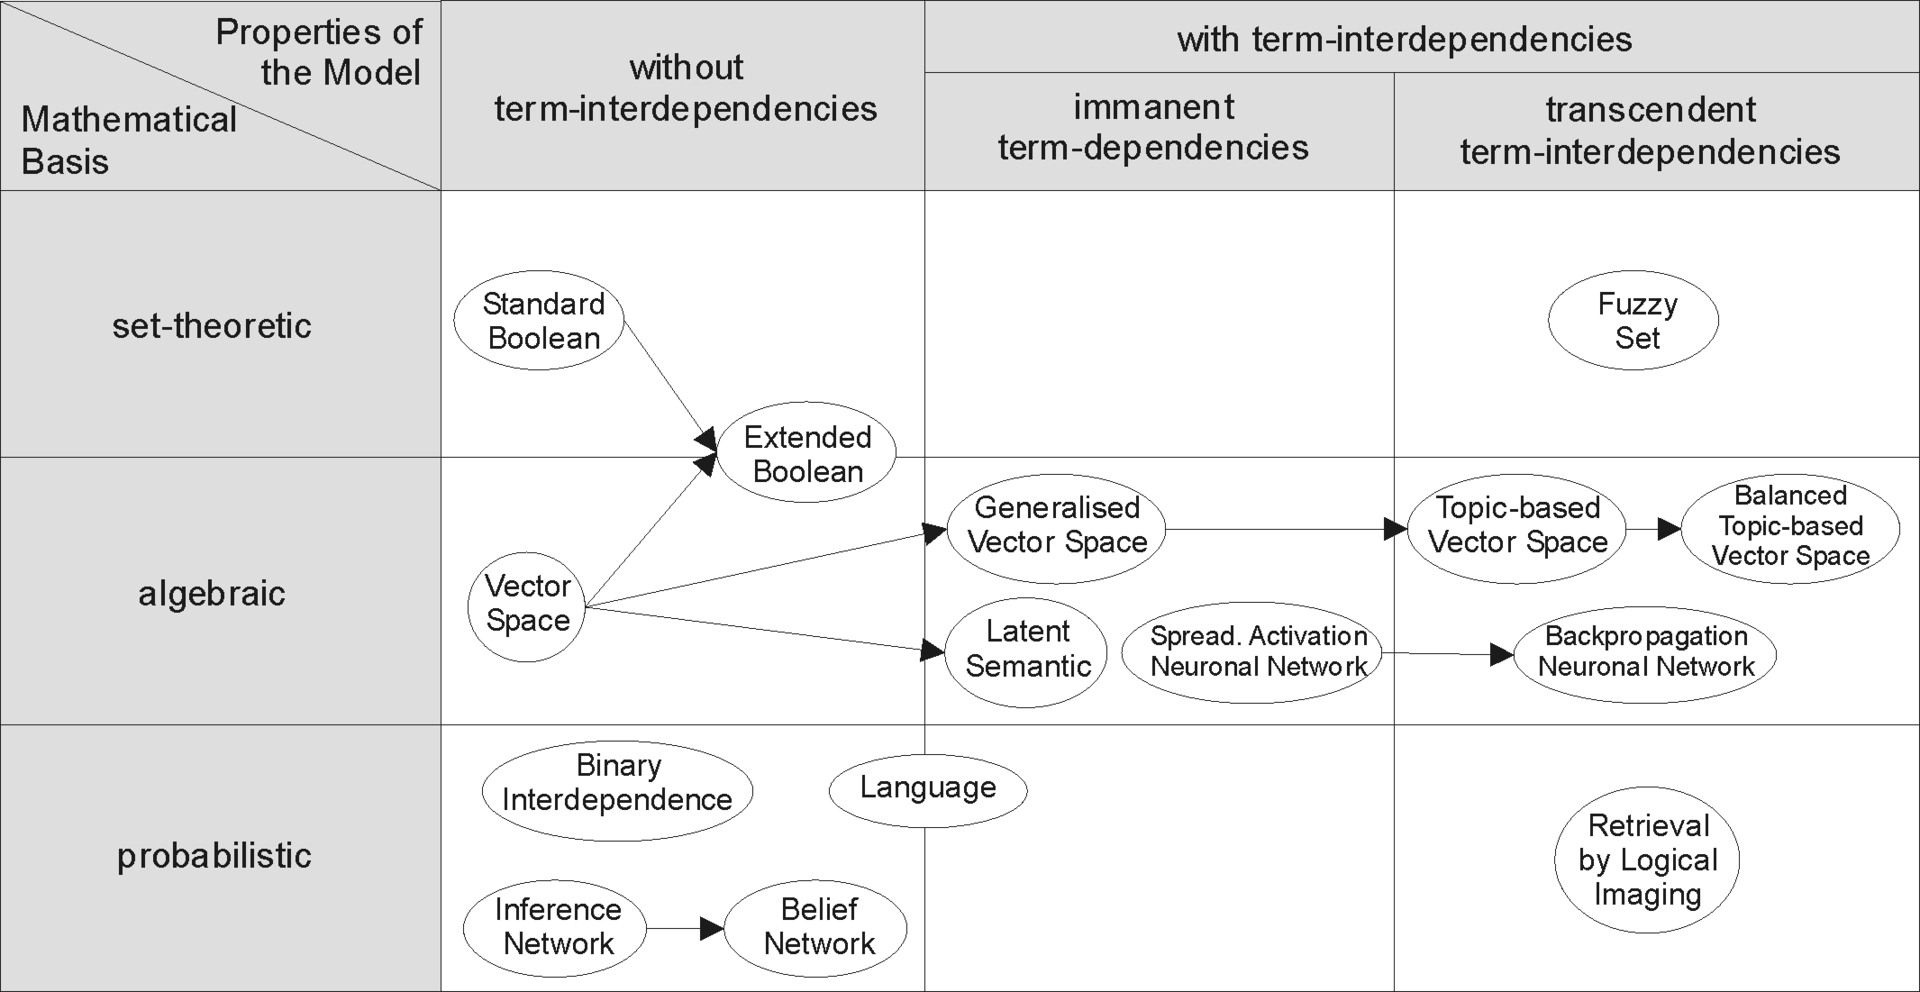
\includegraphics[scale=0.70]{immagini/Information-Retrieval-Models.png}
    \caption{Modelli di recupero dell'informazione}
 \end{figure}
\end{center}
Come rappresentiamo i documenti e interrogazione dipende principalmente del modello di recupero scelto: questo influenza le strategie di recupero e, inevitabilmente, la rappresentazione più conveniente.

Possiamo categorizzare i modelli di recupero in base a:
\begin{itemize}
    \item se viene o meno rappresentata l'interdipendenza tra i termini;
    \item classificazione matematica.
\end{itemize}

Per quanto riguarda lo stage, ci si è limitati ai modelli algebrici: in particolare al modello a spazio vettoriale e al latent semantic indexing.


\subsection{Bag of words}
È un modello di rappresentazione dei documenti che ignora l'ordine dei termini: per ogni termine in un documento, si considera la tupla \textit{<termine, \#occorrenze nel documento>}. 

\subsection{Modello a spazio vettoriale}
Il modello a spazio vettoriale consiste nel rappresentare i documenti e le interrogazioni come dei vettori in uno spazio $|V|$-dimensionale, dove $|V|$ è pari al numero di termini: si tratta, tipicamente di vettori molto sparsi.

\subsection{Definire la distanza tra due documenti}
Per definire la distanza tra due documenti $d$ e $q$ nello spazio vettoriale (o documento e una interrogazione), un'idea potrebbe essere quella di calcolare la loro distanza euclidea.
\begin{equation}
    dist(\mathbf{d},\mathbf{q}) = \sqrt{\sum_{i=1}^n {(d_i-q_i)^2}}    
\end{equation}

Assumiamo che $q$ sia uguale al documento $d$ più il documento $d$ stesso appeso alla fine (quindi due volte $d$): dal punto di vista semantico sono identici, ma la distanza tra i due può essere piuttosto grande e quindi la distanza euclidea è inadatta per misurare la similarità tra due documenti.

Pensando alla rappresentazione a spazio vettoriale, è evidente che $d$ e $q$ manterrebbero comunque lo stesso angolo rispetto l'origine: per valutare la similarità conviene quindi considerare l'angolo, o meglio ancora il coseno, invece che la distanza euclidea.
\begin{equation}
\text{similarità} = \cos(\theta) = {\mathbf{d} \cdot \mathbf{q} \over \|\mathbf{d}\| \|\mathbf{q}\|} = \frac{ \sum\limits_{i=1}^{n}{d_i  q_i} }{ \sqrt{\sum\limits_{i=1}^{n}{d_i^2}}  \sqrt{\sum\limits_{i=1}^{n}{q_i^2}}}
\end{equation}

Questo perché, più due documenti sono simili e più è piccolo l'angolo che li separa, mentre noi vorremmo assegnare un valore più alto all'aumentare della similarità (cosa che succede con il coseno). 

\section{Scoring}
Per misurare l'importanza di un termine rispetto a un documento, vorremmo tenere conto di due fattori:
\begin{itemize}
    \item quante volte il termine compare nel documento (\textbf{term frequency});
    \item l'informatività del termine (\textbf{inverse document frequency}).
\end{itemize}

\subsection{Term frequency}
Rappresenta quante volte il termine compare nel documento:
\begin{equation}
    tf_{t,d} = 1 + log_2(\text{\#occorrenze del termine t nel documento d})
\end{equation}

La rilevanza di un termine non cresce in maniera lineare con l'aumentare del numero delle occorrenze: per questo ci interessa il logaritmo e non il numero delle occorrenze.

\subsection{Inverse document frequency}
Rappresenta l'informatività di un termine:
\begin{equation}
    idf_t = log_2(\frac{\text{\#documenti del corpus}}{\text{\#documenti che contengono il termine t}})
\end{equation}

Un termine raro ci dice molto di più su un documento che uno frequente\footnote{Si veda il concetto di entropia nella teoria dell'informazione: \url{https://en.wikipedia.org/wiki/Entropy_(information_theory)}}; anche in questo caso il logaritmo ci serve per ridurre il valore finale (nei casi in cui il numero dei documenti è elevato).

\subsection{tf-idf}
Si definisce tf-idf di un documento d e un termine d come:
    \begin{equation}
        tf\-idf_{t,d} = tf_{t,f} * idf_{t}
    \end{equation} 

ovvero l'unione tra il numero di occorrenze di un termine in un documento e l'informatività del termine nel documento.

$tf\-idf_{t,d}$ assegna un peso nel documento d che è:
\begin{itemize}
    \item il più alto, quando t compare molte volte in un piccolo numero di documenti;
    \item più basso, quando un termine compare poche volte oppure in molti documenti;
    \item minimo, quando un termine compare praticamente tutti i documenti.
\end{itemize}

\subsection{Matrice termini-documenti}
La nostra collezione di N documenti può essere vista, oltre che come una collezione di N vettori, come una matrice termini-documenti: una matrice le cui righe rappresentano i termini e le colonne i documenti.


\section{Ranking}
Una volta stabilito quali documenti devono vogliamo ritornare da una ricerca, dobbiamo capire come possiamo ordinare i risultati: non tutti i risultati meritano la stessa attenzione da parte dell'utente, che di norma non andrà a controllarli tutti.

Nel caso specifico del progetto, si utilizza Okapi BM25 per lo scoring dei documenti,
Data una interrogazione $Q$, con $q_1, \dots , q_n$ parole chiave, il BM25 score è 

\begin{equation}
    \text{score}(D,Q) = \sum_{i=1}^{n} \text{IDF}(q_i) \cdot \frac{\text{(\#occorrenze di q\textsubscript{i} in D)} \cdot (k_1 + 1)}{\text{(\#occorrenze di q\textsubscript{i} in D)} + k_1 \cdot \left(1 - b + b \cdot \frac{|D|}{\text{avgdl}}\right)}
\end{equation}

dove $|D|$ è il numero di termini nel documenti D, $avgdl$ è lunghezza media dei documenti del corpus, $k_1$ e $b$ parametri liberi.

\section{Tollerant retrieval}
Ammettere una certa tolleranza nel recupero dell’informazione può essere d’aiuto per aumentare la recall (prestando ovviamente attenzione a non peggiorare troppo la precision). Nel caso specifico del progetto, una tipologia d'errore era quella delle parole che suonavano in maniera simile: per esempio "SitePainter" veniva trascritto "serpente".

L’uso di \gls{algoritmi-fonetici} come Soundex, Metaphone e Double Metaphone purtroppo si è rivelato essere inefficace per correggere questi errori. Esiste anche una versione più aggiornata di Metaphone (la 3), ma per motivi di licenza\footnote{Nonostante esista una versione open-source rilasciata con licenza BSD, l'autore della libreria non ne permette il porting in altri linguaggi \url{https://github.com/threedaymonk/text/issues/21\#issuecomment-67752327}} si è preferito non tentare questa strada.

\subsection{Stopwords}
Filtrare le stopword ci può essere d’aiuto nel migliorare la precisione, ma determinare cosa togliere e cosa no non è banale. Un possibile approccio potrebbe essere quello di escludere quei termini che sono uniformemente distribuiti nel corpus (come gli articoli, i pronomi, le preposizioni, le congiunzioni e le interiezioni), ma anche così si rischia di eliminare informazioni solo all'apparenza ininfluenti: esempio classico inglese è "to be or not to be".

\section{Valutazione di un sistema di recupero dell'informazione}
Per riuscire a migliorare il nostro sistema, dobbiamo prima capire come possiamo misurare (e gli eventuali limiti delle misure)

Il nostro sistema ideale dovrebbe:
\begin{itemize}
    \item ritornare tutti i risultati pertinenti;
    \item i risultati ritornati dovrebbero essere tutti pertinenti.
\end{itemize}

Purtroppo l’ideale si scontra con l’ideale e dobbiamo trovare un compromesso tra le due proprietà desiderate: quindi ci interessa capire quanto in sistema di \gls{ir} soddisfa queste due proprietà e a tale scopo definiremo la precision e la recall.


\subsection{Vero positivo, falso positivo, vero negativo, falso negativo}
\begin{center}
    \begin{figure}
        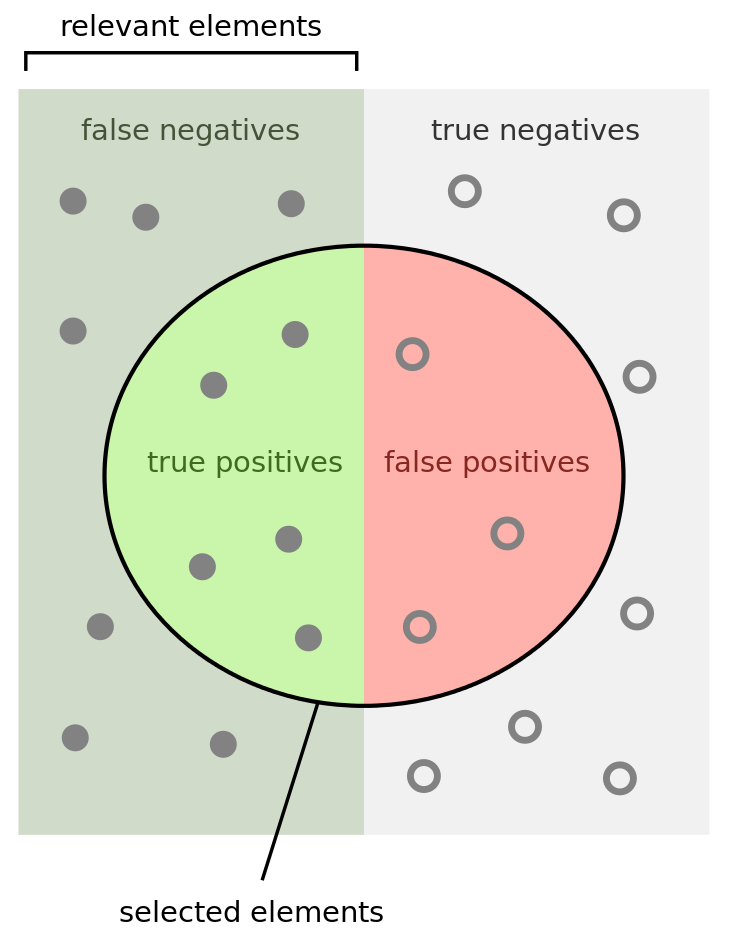
\includegraphics[scale=0.2]{immagini/truefalsenegativepositive.png}
        \caption{Veri/falsi positivi e veri/falsi negativi}
    \end{figure}
\end{center}
Data una interrogazione $q$ e un documento $d$, il risultato dell'interrogazione è un:
\begin{itemize}
    \item \textbf{falso positivo} se il documento $d$ non è rilevante per la ricerca, ma è stato ritornato;
    \item \textbf{vero positivo} se il documento $d$ è rilevante per la ricerca ed è stato ritornato;
    \item \textbf{falso negativo} se il documento $d$ è rilevante per la ricerca, ma non è stato ritornato;
    \item \textbf{vero negativo} se il documento $d$ non è rilevante per la ricerca, e non è stato ritornato;
\end{itemize}

\FloatBarrier

\subsection{Metriche di valutazione}
\label{sub:metriche-valutazione}
\begin{center}
\begin{figure}
    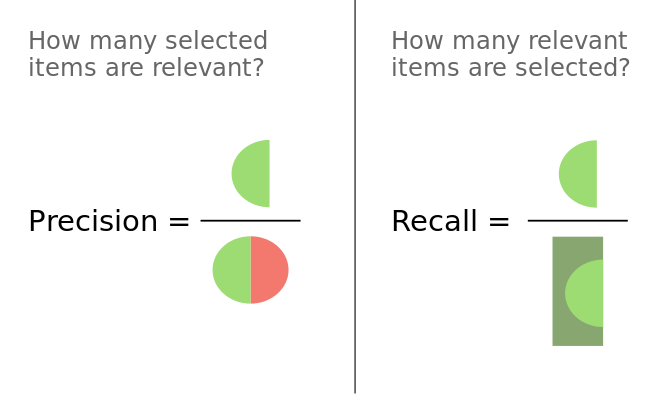
\includegraphics[scale=0.2]{immagini/precisionrecall.png}
    \caption{Precisione e recall}
\end{figure}
\end{center}
\begin{description}
    \item[recall] di una interrogazione a un sistema IR è definita come:
    \begin{equation}
        \mbox{Precisione}=\frac{|\{\mbox{documenti attinenti}\}\cap\{\mbox{documenti recuperati}\}|}{|\{\mbox{documenti recuperati}\}|}
    \end{equation}
    ovvero ci da una misura di quanti dei risultati pertinenti presenti nel corpus siamo riusciti a recuperare e quindi dei falsi negativi di una interrogazione. 
    \item[precision] di una interrogazione a un sistema IR come: 
    \begin{equation}
        \mbox{Recupero}=\frac{|\{\mbox{documenti attinenti}\}\cap\{\mbox{documenti recuperati}\}|}{|\{\mbox{documenti attinenti}\}|} 
    \end{equation}
    ovvero ci da una misura della bontà dei risultati recuperati e quindi della quantità di falsi positivi.
\end{description}
Ambedue sono facilmente riformulabili in termini di vero positivo, falso positivo, vero negativo e falso negativo. Nel decidere a quale delle due dare la priorità, bisogna tenere conto dei due estremi:
\begin{itemize}
    \item per avere una recall pari a 1, è sufficiente ritornare tutti i documenti;
    \item nel cercare di avere una precision tendente a 1, c'è il rischio di essere eccessivamente selettivi. 
\end{itemize}

\begin{description}
    \item[f-measure] Abbiamo quindi bisogno di un buon bilanciamento tra recall e precision. Una misura che sintetizzi le due precedenti è chiamata f-measure e corrisponde alla media armonica tra precision e recall. 
    \begin{equation}
        F_1 = 2 \cdot \frac{\mathrm{precision} \cdot \mathrm{recall}}{\mathrm{precision} + \mathrm{recall}}
    \end{equation}
    
    Calcolare la media aritmetica tra precision e recall sarebbe ancora più facile, ma tale valore sarebbe poco significativo per valutare la bontà della nostra ricerca. (i.e. si potrebbe ritornare sempre l'intero corpus e ottenere sempre una media aritmetica di 0.5)
\end{description}


\FloatBarrier

\subsection{Gold standard} 
Per valutare un sistema di reperimento dell’informazione non è sufficiente valutare come si comporta con rispetto a una interrogazione, ma rispetto a un numero congruo di interrogazioni.
Come rule of thumb, 50 interrogazioni sono considerate un numero congruo, anche se bisogna considerare altri vincoli che cambiano le carte in tavola( nel caso particolare del progetto, era richiesto che le query dovessero contenere falsi positivi, oltre al solito vincolo di avere un corpus piccolo).

Per ogni interrogazione, bisogna quindi segnare quali documenti sono pertinenti (dove, con pertinente, si considera sempre il soddisfacimento o meno del bisogno informativo dell’utente): è il cosiddetto \gls{gold-standard} o ground truth.

Con queste informazioni, è quindi possibile (e facile) calcolare precision, recall e f-measure per ogni interrogazione: purtroppo la costruzione di una gold standard richiede anche parecchio tempo.